\documentclass[../main.tex]{subfiles}
\graphicspath{{\subfix{../images/}}}
\begin{document}

\section{Non right-angle trigonometry}
Given a triangle with no right angles, with sides and angles labelled as below, there are three useful rules that we can use:

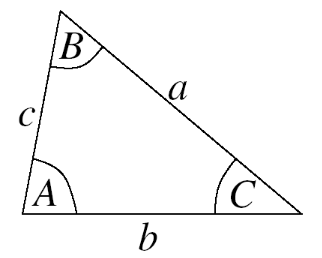
\includegraphics[width=4cm]{images/nonrighttrig.png}

\textbf{Sine Rule}

\(\frac{\sin{A}}{a}=\frac{\sin{B}}{b}=\frac{\sin{C}}{c}\)

\textbf{Cosine Rule}

\(c^2=a^2+b^2-2ab\cos{C}\)

\textbf{Area of triangle}

\(A=\frac{1}{2}ab\sin{C}\)

\pagebreak
\hypertarget{nonrighttriglink}{\subsection*{Questions}}
\hyperlink{nonrighttriganswers}{(Answers - page {\pageref*{Non right trig answers}})}

\label{Non right trig}
Questions go here


\begin{enumerate}
    \item \( (x+y)^3 \)
    \item \( (2x+y)^4 \)
    \item \( (2x-3)^5 \)
    \item \( (3x+2y)^4 \)
    \item \( (2x + \frac{1}{x^2 } )^4 \)
\end{enumerate}






\end{document}